\documentclass[12pt,a4paper,openright]{report}
\usepackage[italian]{babel}
\usepackage{newlfont}
\usepackage[utf8]{inputenc}
\usepackage{fancyhdr}
\usepackage{indentfirst}
\usepackage{showkeys}
\usepackage{amssymb}
\usepackage{amsmath}
\usepackage{latexsym}
\usepackage{amsthm}
\usepackage{qcircuit}
\usepackage{braket}
\usepackage{kbordermatrix}
\usepackage{relsize}
\usepackage{listings}
\usepackage{color}
\usepackage{graphicx}
\usepackage{tikz}
\usepackage{caption}
\captionsetup[figure]{labelformat=empty}
\usetikzlibrary{arrows,shapes.gates.logic.US,shapes.gates.logic.IEC,calc}
\definecolor{dkgreen}{rgb}{0,0.6,0}
\definecolor{gray}{rgb}{0.5,0.5,0.5}
\definecolor{mauve}{rgb}{0.58,0,0.82}
\renewcommand{\chaptermark}[1]{\markboth{\thechapter.\ #1}{}}
\renewcommand{\sectionmark}[1]{\markright{\thesection \ #1}{}}
\newcommand*{\field}[1]{\mathbb{#1}}
\newcommand*\xor{\mathbin{\oplus}}
\newcommand*\Mycomb[2]{\prescript{#1\mkern-0.5mu}{}C_{#2}}
\newcommand{\norm}[1]{\left\lVert#1\right\rVert}
\newtheorem{mydef}{Definizione}[chapter]
\newtheorem{mylem}{Lemma}
\newtheorem*{mycor}{Corollario}
\newtheorem{mythm}{Teorema}[chapter]
\pagestyle{fancy}\addtolength{\headwidth}{30pt}
\rhead[\fancyplain{}{\bfseries\leftmark}]{\fancyplain{}{\bfseries\thepage}}
\cfoot{}


%%%%%%%%%%%%%%%%%%%%%%%%%%%%%%%%%%%%%%%%%
\linespread{1.3}                        %comando per impostare l'interlinea
%%%%%%%%%%%%%%%%%%%%%%%%%%%%%%%%%%%%%%%%%definisce nuovi comandi
%
\textwidth=450pt\oddsidemargin=0pt
\begin{document}
\begin{titlepage}
\begin{center}  
{{\Large{\textsc{Alma Mater Studiorum $\cdot$ Universit\`a di
Bologna}}}} \rule[0.1cm]{15.8cm}{0.1mm}
\rule[0.5cm]{15.8cm}{0.6mm}
{\small{\bf SCUOLA DI SCIENZE\\
Corso di Laurea in Informatica }}
\end{center}
\vspace{15mm}
\begin{center}
{\LARGE{\bf TITOLO}}\\
\vspace{3mm}
{\LARGE{\bf DELLA}}\\
\vspace{3mm}
{\LARGE{\bf TESI}}\\
\end{center}
\vspace{40mm}
\par
\noindent
\begin{minipage}[t]{0.47\textwidth}
{\large{\bf Relatore:\\
Chiar.mo Prof.\\
UGO DAL LAGO}}
\end{minipage}
\hfill
\begin{minipage}[t]{0.47\textwidth}\raggedleft
{\large{\bf Presentata da:\\
FEDERICO PECONI}}
\end{minipage}
\vspace{20mm}
\begin{center}
{\large{\bf II Sessione\\%inserire il numero della sessione in cui ci si laurea
a.a. 2016/2017 }}%inserire l'anno accademico a cui si è iscritti
\end{center}
\newpage
\thispagestyle{empty}                   %elimina il numero della pagina
\topmargin=6.5cm                        %imposta il margina superiore a 6.5cm
\raggedleft                             %incolonna la scrittura a destra
\large                                  %aumenta la grandezza del carattere
                                        %   a 14pt
\em                                     %emfatizza (corsivo) il carattere
Questa \`e la \textsc{Dedica}:\\
ognuno pu\`o scrivere quello che vuole, \\
anche nulla \ldots                      %\ldots lascia tre puntini
\newpage                                %va in una pagina nuova
%
%%%%%%%%%%%%%%%%%%%%%%%%%%%%%%%%%%%%%%%%
\clearpage{\pagestyle{empty}\cleardoublepage}%non numera l'ultima pagina sinistra
\end{titlepage}
\tableofcontents
\chapter{Introduzione}
\chapter{Funzioni Booleane Bilanciate}
Come già anticipato nell'Introduzione, le funzioni Booleane bilanciate sono una struttura matematica su cui poggia parte del contenuto di questa tesi.
É risultato perciò utile, ai fini di una trattazione chiara ed esaustiva, impiegare un capitolo per definirne in maniera rigorosa i concetti di base.\\
"\textit{Per fare un tavolo ci vuole il legno}" recita l'inizio di una famosa canzone per bambini, ad indicare la natura celata delle cose che, così nella quotidianità
come nella matematica, spesso necessitano di altre conoscenze per essere comprese appieno; seguendo quindi questa impronta fondazionale, andiamo per prima cosa ad introdurre le funzioni Booleane.

\section{Funzioni Booleane}
Le funzioni Booleane apparvero per la prima volta a metà 19esimo secolo durante la formulazione matematica di problemi logici e prendono
il loro nome da George Boole, matematico britannico considerato fondatore della logica matematica odierna\cite{ref2}.\newpage
Una semplice funzione Booleana può può essere rappresentata da \\$f:\{0,1\}^2 \mapsto \{0,1\}$
\begin{align*}  
    f(00) = 0 \\
    f(01) = 0 \\
    f(10) = 1 \\
    f(11) = 0
\end{align*}
oppure da $f^\prime:\{TRUE,FALSE\}\mapsto{\{TRUE,FALSE\}}$
\begin{align*}
    f^\prime(FALSE) = TRUE \\
    f^\prime(TRUE) = FALSE 
\end{align*}
Notiamo come entrambe abbiano in comune la dimensione del codominio e la capacità di agire su un numero finito di valori appartenenti ad un insieme di 2 elementi.
È tuttavia conveniente operare su di un insieme che possa essere visto sia dal punto di vista qualitativo (vero, falso)
sia da un punto di vista quantitativo, e quindi numerico, che ci permetta così di compiere anche operazioni algebriche oltre che logiche. Prediligeremo allora da qui in avanti l'inisieme
$\{0,1\}$ come campo vettoriale su cui lavorare.
\par
\begin{mydef}
    Una \textnormal{funzione Booleana a \textit{n} variabili} è una funzione da $\mathcal{B}^n$ a $\mathcal{B}$,
    dove $\mathcal{B} = \{0,1\}$, $n > 0$ e $\mathcal{B}^n$ è l'n-esimo prodotto cartesiano di $\mathcal{B}$ con se stesso.\cite{ref3}
\end{mydef}
\begin{mycor}
    $\forall$ $n > 0$, ci sono $2^{2^{n}}$ funzioni da $\mathcal{B}^n$ a $\mathcal{B}.$
\end{mycor}
\begin{proof}
    Sia $\mathcal{F}=\{f|f:\mathcal{B}^n\mapsto{\mathcal{B}}\}$,
    ogni $f$ riceve in input n-uple $\vec{x}=(x_1,..,x_n)$ che possono essere viste come sequenze di $n$ bit.
    In $n$ bit possiamo codificare, trattandosi di una distribuzione con ripetizione di classe $n$, $2^n$ oggetti differenti, quindi $\mathbb{D}_{2,n}=\left\vert{\mathcal{B}^n}\right\vert = 2^n$.
    Per definizione di $f$, per ogni $\vec{x}$, $f(\vec{x}) = 0$  oppure  $f(\vec{x}) = 1$, quindi ogni possibile $f$ individua un sottoinsieme di $\mathcal{B}^n$.\\
    Allora $\mathcal{F}$ avrà caridinalità uguale all'insieme delle parti per $\mathcal{B}^n$, quindi  $\left\vert{\mathcal{F}}\right\vert = 2^{\mathcal{B}^n}=2^{2^{n}}$

\end{proof}
Un altro modo più tradizionale per descrivere una funzione Booleana è quello di fornire la sua tabella di verità.
Ad esempio, per la $f$ precedentemente definita, la tabella di verità relativa sarà:


\begin{displaymath}
    \begin{array}{|c|c|c|}\hline
        x_1 & x_2 & f(x_1, x_2) \\\hline 
        0   & 0   &  0  \\ 
        0   & 1   &  0  \\
        1   & 0   &  1  \\
        1   & 1   &  0  \\\hline
    \end{array}
\end{displaymath}
Dove a destra viene posto il risultato della funzione calcolata sui valori delle colonne precedenti.\par
In entrambe le rappresentazioni, tuttavia, le funzioni vengono descritte in maniera implicita mostrando solamente input ed output,
senza mai andare a specificare come questo output venga calcolato.\\
Nell'ultimo capitolo, per l'implementazione dell'algoritmo di Deutsch-Jozsa, verranno utilizzate funzioni Booleane \textit{bilanciate}
che necessitano di essere calcolate esplicitamente. La prossima sezione introduce questa categoria di funzioni Booleane e 
propone due metodi effettivi e generali per produrne istanze concrete.

\section{Classi di Funzioni Booleane Bilanciate}

Sia $f$ una funzione Booleana, chiamiamo $\vec{x}=(x_1,..,x_n)$ \textit{vettore positivo} per $f$ se e solo se
$f(\vec{x}) = 1$, \textit{vettore negativo} altrimenti. Sia $({\left\vert{f}\right\vert}^1 \text{,} {\left\vert{f}\right\vert}^0)$ la partizione dove ${\left\vert{f}\right\vert}^1$ è la quantità che indica il numero di vettori
positivi per $f$ e ${\left\vert{f}\right\vert}^0$ la quantità che indica il numero di vettori negativi.
\begin{mydef}
    Una funzione Booleana $f$ è detta bilanciata (FBB) se e solo se ${\left\vert{f}\right\vert}^1 = {\left\vert{f}\right\vert}^0$.
\end{mydef}
\begin{mycor}
    $\forall$ $n > 0$, ci sono $\frac{2^{n}!}{(2^{n-1}!)^2}$ FBB da $\mathcal{B}^n$ a $\mathcal{B}.$
\end{mycor}
\begin{proof}
    Per definizione, una FBB $fbb:\mathcal{B}^n\mapsto\mathcal{B}$ è individuata da una partizione $(\mathcal{M},\mathcal{N})$ con $\mathcal{M}\subset\mathcal{B}^n$ e $\mathcal{N}\subset\mathcal{B}^n$ tale che
    $\left\vert{\mathcal{M}}\right\vert = \left\vert{\mathcal{N}}\right\vert = 2^{n-1}$ e $fbb(m)=0 \land fbb(n)=1$ $\forall{m,n}$ con $m\in\mathcal{M},n\in\mathcal{N}$.
    Quindi, il numero delle possibili funzioni corrisponde a tutti i possibili modi di partizionare a metà un insieme di $2^n$ elementi e, a sua volta, ogni partizione così creata può essere rappresentata 
    da un sottoinsieme $\mathcal{S}\subset\mathcal{B}^n$ dove $\mathcal{M}=\mathcal{S}$ e $\mathcal{N}=\mathcal{B}^n \setminus \mathcal{S}$.
    Non resta quindi che trovare tutti i possibili $\mathcal{S}$:  
    \begin{center}
    \[
        \mathbb{C}_{2^n,2^{n-1}}= \binom{2^n}{2^{n-1}} = \frac{2^n!}{2^{n-1}!2^{n-1}!} = \frac{2^n!}{(2^{n-1}!)^2}
    \]
    \end{center}
\end{proof}
Una valida tabella di verità per una FBB in $\mathcal{B}^3$ portebbe essere la seguente:

\begin{center}
\scalebox{0.90}{$
    \begin{array}{|c|c|}\hline
        (x_1,x_2,x_3) & g(x_1,x_2,x_3) \\\hline 
        (0,0,0)         &  0  \\ 
        (0,0,1)         &  1  \\
        (0,1,0)         &  1  \\
        (0,1,1)         &  0  \\    
        (1,0,0)         &  1  \\
        (1,0,1)         &  0  \\
        (1,1,0)         &  0  \\
        (1,1,1)         &  1  \\\hline
    \end{array}$
}
\end{center}
Dove, giustamente, si noti come il numero dei vettori positivi equivale al numero dei vettori negativi.\par
Ma come è costruita $g$ nello specifico? Qual'è la computazione che mi porta a determinati outputs?
Per rispondere a queste domande si può provare a cercare qualche correlazione tra i valori in entrata e i valori in uscita:
dopo un pò di riflessione dovrebbe saltare all'occhio che ogni qual volta abbiamo un numero dispari di $1$ nell'input la funzione 
restituisce $1$, restituisce invece $0$ quando tale numero è pari.
La parità di una sequenza è esprimibile con la somma modulo $2$ dei singoli componenti, allora possiamo definire esplicitamente $g$ come:
\begin{align*}
    g(x_1, x_2, x_3)= &x_1 + x_2 + x_3 \mod 2  \\
                    = &(x_1 \xor x_2) \xor x_3  \\
                    = &x_1 \xor x_2 \xor x_3
\end{align*}
dove $\xor$ è un connettivo binario logico (una funzione Booleana $\in \mathcal{B}^2$) chiamato XOR oppure OR esclusivo, che restituisce $1$ se uno ed uno solo dei due 
elementi vale $1$. 

\begin{center}
    \scalebox{0.90}{$
        \begin{array}{|c|c|}\hline
            (x_1,x_2) & \xor(x_1,x_2) \\\hline 
            (0,0)         &  0  \\ 
            (0,1)         &  1  \\
            (1,0)         &  1  \\
            (1,1)         &  0  \\\hline    
        \end{array}$
    }
    \end{center}
\par
\begin{mylem}
    Per ogni $n > 0$ la funzione Booleana $ f^{n}(x_1,x_2,...,x_n) = x_1 \xor x_2 \xor ... \xor x_n $ è una FBB.  
\end{mylem}
\begin{proof}
    \textit{(per induzione su $n$)\\}
    \begin{description}
        \item[Base induttiva:] $f^1(x)=x$ è trivialmente bilanciata.
        \item[Ipotesi induttiva:] Ipotizziamo $f^n$ bilanciata, quindi esiste la partizione $(\mathcal{M},\mathcal{N})$ con $\mathcal{M}\subset\mathcal{B}^n$ e $\mathcal{N}\subset\mathcal{B}^n$ tale che:\\
                                      ${\left\vert{\mathcal{M}}\right\vert} = {\left\vert{\mathcal{N}}\right\vert}$, $\mathcal{M} \cup \mathcal{N} = \mathcal{B}^n$ e $\forall m,n$ con
                                      $m\in\mathcal{M}$,$n \in\mathcal{N}$ risulta $f^n(m) = 0$ e $ f^n(n) = 1$.
        \item[Passo induttivo:] Avremo $f^{n+1}:\mathcal{B}^{n+1}\mapsto\mathcal{B}$ dove  $\mathcal{B}^{n+1} = \mathcal{B}^n\cdot0 \cup \mathcal{B}^n\cdot1$ e quindi\\
                                     $\left\vert\mathcal{B}^{n+1}\right\vert = 2\left\vert\mathcal{B}^{n}\right\vert$. Dobbiamo dimostrare che esiste una partizione
                                     $(\mathcal{M^\prime},\mathcal{N^\prime})$ t.c.:
                                     \begin{itemize}
                                        \item $\left\vert\mathcal{M^\prime}\right\vert=\left\vert\mathcal{B}^{n}\right\vert$ e $\forall m^\prime \in \mathcal{M^\prime}$ $f^{n+1}(m^\prime) = 0$ 
                                        \item $\left\vert\mathcal{N^\prime}\right\vert=\left\vert\mathcal{B}^{n}\right\vert$ e $\forall n^\prime \in \mathcal{N^\prime}$ $f^{n+1}(n^\prime) = 1$   
                                      \end{itemize}
                                      Notiamo come, $\forall m,n$ con $ m\in\mathcal{M},n\in\mathcal{N}$ se\\
                                      $x_{n+1} = 0 \Rightarrow $ $f^{n+1}(m\cdot0)=0 \land f^{n+1}(n\cdot0)=1$\\
                                      $x_{n+1} = 1 \Rightarrow $$f^{n+1}(m\cdot1)=1 \land f^{n+1}(n\cdot1)=0$\\
                                      Segue naturalmente che la partizione $\mathcal{M^\prime} = \mathcal{M}\cdot0 \cup \mathcal{N}\cdot1$ e $\mathcal{N^\prime} = \mathcal{M}\cdot1 \cup \mathcal{N}\cdot0$
                                      rispetta i criteri cercati. 
    \end{description}      
\end{proof}
\par
Si richiami dall'Algebra Lineare che, $f:\mathcal{V}\mapsto\mathcal{W}$ è un'applicazione lineare se e solo se esiste una matrice $M \in \mathbb{M}^{k \times l}$ tale che $f(\vec{x})=M\vec{x}$, dove $k = \left\vert\mathcal{V}\right\vert$ e $l = \left\vert\mathcal{W}\right\vert$ sono le dimensioni degli spazi vettoriali su cui agisce.\\

\begin{mydef}
$b:\mathcal{B}^n \mapsto \mathcal{B}$ è una funzione booleana lineare (FBL) se e solo se esiste $M \in \mathbb{B}^{n \times 1}$ tale che $b(\vec{x})=M\vec{x}=c_1x_1+c_2x_2+,...,+c_nx_n=(c_1\land{x_1})\xor(c_2\land{x_2})\xor,...,\xor(c_n\land{x_n})$. Dove $\xor$
è l'operatore di somma per $\mathcal{B}^n$. 
\end{mydef}
\begin{mycor}
    Per ogni $n>0$, $f^n$ è una FBL.
    \begin{proof}
        Triviale, basta infatti porre $M=\overbrace{(1,1,...,1)}^{n-volte}$.
    \end{proof}
\end{mycor}

\subsection{La Classe delle Funzioni Booleane Lineari}
Introdotte le FBB e le FLB, possiamo a questo punto procedere con la formulazione del seguente risultato generale:
\begin{mythm}
    Sia $\mathbb{FL}=\{f|f\in\text{FLB} \land f \neq c:\mathcal{B}^n\mapsto\{0\},\;\forall n > 0\}$ la classe di tutte le funzioni Booleane lineari
    diverse dalle funzioni costanti a 0. Allora, $\forall f\in \mathbb{FL}$ $f$ è bilanciata.
\end{mythm}
\begin{proof} \textit{(per induzione su $n$)\\}
    Sia $l^n$ una qualsiasi funzione da $\mathcal{B}^n$ appartenente a $\mathbb{FL}$.  Vogliamo dimostrare che $l^n$ è sempre bilanciata.\\
    \begin{description}
        \item[Base induttiva:] $l^1(x)=x$ è trivialmente bilanciata.
        \item[Ipotesi induttiva:] Ipotizziamo $l^n$ bilanciata.\\
                                      Esisterà quindi la partizione $(\mathcal{M},\mathcal{N})$ con $\mathcal{M}\subset\mathcal{B}^n$ e $\mathcal{N}\subset\mathcal{B}^n$ tale che:\\
                                      ${\left\vert{\mathcal{M}}\right\vert} = {\left\vert{\mathcal{N}}\right\vert}$, $\mathcal{M} \cup \mathcal{N} = \mathcal{B}^n$ e $\forall m,n$ con
                                      $m\in\mathcal{M}$,$n \in\mathcal{N}$ risulta $l^n(m) = 0$ e $ l^n(n) = 1$.
        \item[Passo induttivo:] Il passo chiave sta nel notare che $l^{n+1}$ può assumere esclusivamente una delle seguenti forme:
                                \begin{itemize}
                                    \item \textbf{Singoletto} $\Rightarrow$ $l^{n+1}(\vec{x}) = l^{n+1}(x_1,x2,...,x_{n+1})=x_{n+1}$\\
                                                              Che è bilanciata in quanto, sia $(\mathcal{M},\mathcal{N})$ la partizione dove $\mathcal{M}$ è composto da tutte le stringhe
                                                              binarie $\in \mathcal{B}^{n+1}$ che codificano in base due i numeri da $0$ a $2^n - 1$ e $\mathcal{N}$ composto da tutte le stringhe binarie
                                                              $\in \mathcal{B}^{n+1}$ che codificano in base due i numeri da $2^n$ a $2^{n+1} - 1$ i.e. :\\
                                                              $\mathcal{M}= \{\vec x \in \mathcal{B}^{n+1} | \vec x = 0\cdot x_n \cdot x_{n-1}\cdot ...\cdot x_1\}$\\
                                                              $\mathcal{N}= \{\vec x \in \mathcal{B}^{n+1} | \vec x = 1\cdot x_n \cdot x_{n-1}\cdot ...\cdot x_1\}$\\
                                                              Allora $\mathcal{M}\subset\mathcal{B}^{n+1}$ e $\mathcal{N}\subset\mathcal{B}^{n+1}$, ${\left\vert{\mathcal{M}}\right\vert} = {\left\vert{\mathcal{N}}\right\vert}$, $\mathcal{M} \cup \mathcal{N} = \mathcal{B}^{n+1}$ e
                                                              e $\forall m,n$. $m\in\mathcal{M}$,$n \in\mathcal{N}$ risulta $l^{n+1}(m) = 0$ e $ l^{n+1}(n) = 1$.
                                    \item \textbf{Uguale a $l^n$} $\Rightarrow$ Bilanciata per ipotesi. 
                                    \item \textbf{Xor di $l^n$} $\Rightarrow$ $l^{n+1}(\vec{x}) = l^{n+1}(x_1,x2,...,x_{n+1})= x_{n+1} \xor l^n$.
                                    \\ E quindi se:\\
                                    $x_{n+1} = 0 \Rightarrow l^{n+1} = 0 \xor l^n = l^n$ \\
                                    $x_{n+1} = 1 \Rightarrow l^{n+1} = 1 \xor l^n = \neg l^n$\\
                                    Individuiamo, concludendo la dimostrazione, la partizione cercata $(\mathcal{M^\prime},\mathcal{N^\prime})$ con:\\
                                    $\mathcal{M^\prime} = M\cdot0 \cup N\cdot1 \:\:$  e  $\:\: \mathcal{N^\prime} = M\cdot1 \cup N\cdot0$.
                                \end{itemize}
    \end{description}
\end{proof}
\noindent Questo significa che, qualsiasi siano i coefficienti della nostra FBL, a patto che questi non siano tutti $0$, produrrano una funzione bilanciata.\par

Giunti a questo punto è lecito domandarsi se esistano altre (semanticamente diverse) FBB  non lineari e se sì, quante ne si possono ancora trovare?
Il numero di FBL per $n$ fissato, equivale al numero di \textit{disposizioni con ripetizione di classe} $n$ (coefficienti) da un insieme di due elementi $\{0,1\}$ meno la disposizione $M^*=\overbrace{(0,0,...,0)}^{n-volte}$ che identifica la costante 0, cioè $\mathbb{D}_{2,n}-1= 2^n - 1$.
Tale numero è chiaramente inferiore al numero di FBB : $\mathbb{C}_{2^n,2^{n-1}}$ ricavato dal Corollario 2.2. E quindi sì, esisteranno sicuramente, per ogni $n$, $\mathbb{C}_{2^n,2^{n-1}} - (\mathbb{D}_{2,n} - 1)$ FBB non lineari.

\subsection{Funzioni Booleane non Lineari Bilanciate}
L'approfondimento delle proprietà e della teoria riguardante il vasto campo di studi delle funzioni Booleane, per quanto interessante, esula dai fini della tesi in oggetto.
Rimanendo in tema, tuttavia, è bene accennare che la ricerca, specie per quanto riguarda l'indagine sulle funzioni booleane bilanciate è molto attiva e di fondamentale importanza in applicazioni come la crittografia a chiave simmetrica.\cite{ref4}.\\
Per rendere più realistica e articolata l'implementazione degli script presentati nel Capitolo 5, si è optato per la ricerca in letteratura di funzioni booleane bilanciate non lineari
da utilizzare nell'algoritmo di Deutsch-Jozsa. In particolare, è stata scelta una funzione a 5 variabili, ricavata con il metodo generale esposto da \textit{Logachev}\cite{ref5}:
    \begin{align*}
            h(x_1, x_2, x_3, x_4, x_5)=(x_1 \land x_2) \xor x_3 \xor (x_2 \land x_3 \land x_4) \xor (x_2 \land x_3 \land x_5) \xor (x_3 \land x_4) \xor (x_4 \land x_5)
    \end{align*}



\begin{figure}[h]
     \centering
     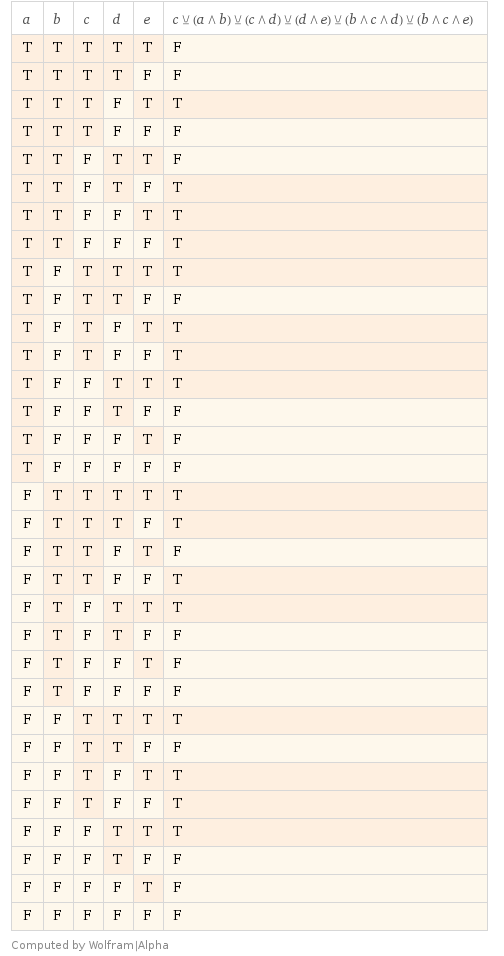
\includegraphics[width=0.5\textwidth,height=13.1cm]{computedFBBtrueTable}
     \caption{Tabella di verità per $h$}
\end{figure}
    

\chapter{L'Informazione Quantistica}
Questa tesi si sviluppa nel contesto dell'Informazione Quantistica.\\
L'Informazione Quantistica è una nuova branca di studi della teoria dell'informazione che trova la sua collocazione nell'intersezione tra
Fisica, Matematica e Informatica.\\
La nascita di questo nuovo campo di studi è dovuta in gran parte alle intuizioni del celeberrimo fisico Richard Feynmann, il quale fu il primo a suggerire,
in una sua lezione nel 1981 \cite{ref6}, che il tipo di computer ideale che fosse stato capace di simulare i fenomeni fisici in maniera
efficiente sarebbe stato solo un computer che avesse risposto alle stesse leggi della meccanica quantistica. L'argomento da lui proposto faceva
perno sulla natura esponenziale che il mondo subatomico presenta se osservato dal punto di vista macroscopico e che quindi, avrebbe portato,
per un processo transitivo, qualsiasi computer classico a sperimentare un tempo altrettanto esponenziale per simularlo.\\
Spinti da questa osservazione, numerosi ricercatori si cimentarono nello studio e nella formalizzazione di questo nuovo paradigma di calcolo,
gettandone le basi teoriche: nel 1982, Paul Benioff, nell'articolo "Quantum mechanical models of Turing machines that dissipate no energy"\cite{ref7}, 
dimostrò come un sistema basato sulla meccanica quantistica avrebbe potuto modellare una macchina di Turing (MdT) senza dissipare energia (il concetto della conservazione dell'energia 
verrà ripreso e chiarito in seguito). In altre parole, questi dimostrò come la fisica dei quanti fosse sufficiente ad esprimere un qualsiasi modello tradizionale di calcolo; ma poteva addirittura fare di meglio? \\
All'incirca nello stesso periodo, il fisico David Deutsch rispose a tale quesito \cite{ref12} introducendo prima la controparte quantica della MdT universale (QMdTU)
e poi dimostrando che la QMdTU riusciva a compiere operazioni al di fuori della portata della MdTU, come generare in maniera genuina numeri random,
performare calcoli paralleli su di un unico registro e simulare perfettamente in tempo polinomiale sistemi fisici a stati di dimensione finita, confermando così
la visionaria congettura che Feynmann aveva sollevato solo pochi anni prima.  

\section{Principi della Meccanica Quantistica}
Nel mondo microscopico, quando si scende sotto la soglia atomica, cominciano ad emergere fenomeni che sono difficilmente interpretabili utilizzando il solo senso comune.
Le nozioni più elementari come la determinazione unica delle proprietà fisiche di un oggetto (velocità, posizione, ecc.) a cui siamo abituati fin da piccoli non sono più le stesse e,
postulati come il principio di località o il determinismo, cessano di essere veri.
Ciò portò inizialmente eminenti fisici del tempo a guardare con scetticismo o addirittura a rifiutare la meccanica quantistica per via delle stranezze a cui essa portava,
numerosi esperimenti condotti successivamente hanno tuttavia confermato con successo le previsioni di questa e, ad oggi, nella comunità scientifica vi è unanime consenso sulla veriditicità fenomenica della meccanica quantistica.\\
Al fine di capire il calcolo quantistico è necessario per prima cosa acquisire familiarità con le nuove leggi fondamentali che governano il mondo infinitamente piccolo.
Vengono quì esposte sinteticamente le caratteristiche peculiari della fisica quantistica e, di seguito in maniera più formale, il modo in cui influenzano l'informatica.

\subsection{Dai Numeri Reali ai Numeri Complessi}
La meccanica quantistica differisce dalla maggior parte delle branche della scienza per via del largo uso che fa dei numeri complessi.
I numeri complessi vennero per la prima volta introdotti come una curiosità matematica: $i=\sqrt{-1}$, chiamata unità immaginaria, era la soluzione "immaginaria" postulata
all'equazione $x^2=-1$. Per tanto tempo il campo dei numeri complessi è rimasto confinato unicamente nel reame della matematica fino a quando,
con lo studio sistematico delle funzioni d'onda e l'introduzione delle analisi di Fourier, ci si accorse che i numeri complessi erano la struttura
ottimale per descrivere in maniera compatta un'onda. Inizialmente la meccanica quantistica fece largo uso delle funzioni d'onda.\par
\begin{mydef}
    Un numero complesso $\text{c}$ è un'espressione
    \begin{center}
        $c = a + b \times i = a + bi$\\
    \end{center}
        dove $a$ e $b$ sono due numeri reali, $a$ è chiamata la parte reale di $c$, mentre $b$ è la parte immaginaria.
    
\end{mydef}


\subsection{Da Stati Singoli alla Sovrapposizione degli Stati}
  Contrariamente a quello che abbiamo imparato fin da piccoli osservando il mondo in cui viviamo, un oggetto subatomico può trovarsi contemporaneamente in più posizioni differenti.\\
  Questo comportamento, detto di sovrapposizione, è tradizionalmente esemplificato riportando l'esperimento \cite{ref13} delle due fenditure attraverso cui viene 
  fatta passare, una alla volta, una qualsiasi particella che andrà a sbattere contro un rilevatore posto dietro le fenditure. Contrariamente a quanto verrebbe da pensare,
  il rilevatore non rileva come colpite dalle particelle solo le due aree in linea con le fenditure (e.g. come accadrebbe per dei palloni calciati in una porta coperta a meno di due sottoporte) bensì vengono 
  sperimentalmente rilevate diverse aree di collisione, ognuna delle quali è colpita con un'intensità diversa, seguendo una distribuzione ad interferenza.
  Ogni singola particella discreta si comporta anche come un'onda che, passando \emph{contemporaneamente} per le due fessure, interferisce poi con se stessa.
  La dualità onda particella della materia scoperta grazie ai lavori di Luis de Broglie, Max Planck e altri fisici del secolo scorso, fu un risultato d'importanza cardinale per l'avvento della meccanica quantistica.
  Non solo la spazialità, ma anche altre proprietà come l'energia, il momento e lo spin di una particella sono soggette a sovrapposizione.\\
  In realtà, non è possibile osservare direttamente il processo di sovrapposizione di una proprietà poichè, ogni qual volta viene effettuata una misurazione su di un
  sistema quantistico, questo verrà alterato inevitabilmente seguendo il principio di indeterminazione di Heisenberg e collasserà in uno ed uno solo degli stati sovrapposti, seguendo, come verrà chiarito più avanti, una ben definità distribuzione di probabiltà.\\
  La sovrapposizione è il principale effetto che viene sfruttato per ottenere vantaggi computazionali. 
\begin{figure}[h]
    \centering
    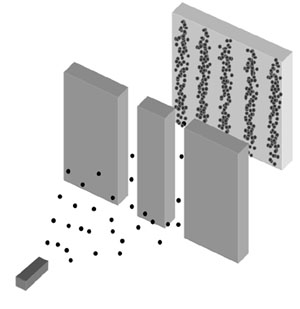
\includegraphics[width=0.5\textwidth]{double-slit-electrons1}
    \caption{visualizzazione dell'esperimento delle due fenditure}
\end{figure}
  
\subsection{Dalla Località alla non Località}
Centrale nella scienza moderna è la nozione secondo cui due oggetti, in un sistema, si influenzano tra di loro secondo un rapporto di causa-effetto solo se essi
sono connessi da un'interazione fondamentale. La velocità di propagazione di una qualsiasi interazione è soggetta al limite imposto dalla velocità della luce 
nel vuoto, per cui non esisteranno due oggetti che, posti all'interno dello stesso sistema entrino in relazione immediatamente. Questa assunzione, 
che prende il nome di principio di località, non è sempre valida nella fisica quantistica. È possibile infatti
mettere due particelle in una relazione chiamata \emph{entanglement} (le due particelle si diranno entangled) tale per cui non sia più possibile
descriverne il comportamento in maniera separata facendo si che, qualsiasi  operazione compiuta su di una avrà un effetto immediato su l'altra, 
indipendentemente dalla loro distanza.    

\subsection{Dalle leggi Deterministiche a quelle Non Deterministiche}
Verso quale specifico stato collasserà una sovrapposizione di stati quando misurata? Mentre in altre aree della fisica le leggi sono deterministiche 
i.e. vi è un unico ouput se ripetiamo lo stesso esperimento più volte sotto le stesse condizioni, le leggi della meccanica quantistica
ci dicono, tuttavia, che possiamo solamente conoscere la probabilità con cui un output, e non un altro, si verificherà. \par

Queste azioni, parafrasando Einstein stesso "terrificanti" \footnote{"spooky action at distance" è la famosa frase che utilizzò per descrivere l'entanglement} che emergono nel reame della meccanica quantistica, per quanto radicali ed avulse
dalla nostra esperienza quotidiana, sono poi le stesse, riflettendo la natura esponenziale del mondo sub atomico, che conferiscono all'Informazione quantistica il suo vero potenziale. 

\section{I Sistemi a Confronto}
Per vedere come la meccanica quantistica influenza l'informatica cominciamo presentando un modello per il calcolo che metta in luce 
le differenze quando applicato a più paradigmi differenti. In particolare vengono qui in ordine introdotti i concetti fondamentali 
del calcolo classico, del calcolo probabilistico e infine del calcolo quantistico.
\subsection{Il Reame Classico}

\subsubsection{Il Bit}
L'unità fondamentale su cui si fonda il calcolo classico è il bit. Consideriamo bit un qualsiasi sistema che 
espone un'unica proprietà osservabile che può assumere solo due valori. Chiamiamo questi 2 valori $\ket0$, $\ket1$ \footnote{cominciamo, senza alterarne il significato, ad utilizzare la notazione bra-ket introdotta dal fisico britannico Paul Dirac}.
Per essere coerentemente osservabili, $\ket0$ e $\ket1$ devono avere una precisa implementazione, ad esempio, se il bit è indicato
da un transistor: $\ket0$ può essere identificato dalla presenza di un flusso di elettricità di un certo valore attraverso il transistor mentre
$\ket1$ è identificato dall'assenza di corrente. Altre implementazioni che sfruttino la stessa logica sono ovviamente valide. 
Come già anticipato nel primo capitolo, $\ket0$ e $\ket1$ sono sufficienti per modellare una qualsiasi
funzione booleana e più in generale, un bit è l'unità fondamentale che governa ogni possibile
operazione su un computer moderno.

\subsubsection{Stati e Osservazioni}

Una visione usuale dei sistemi di computazione, e dei sistemi in generale, è quella in cui viene specificato lo spazio dei possibili
stati $\mathcal{B}_s$ in cui è possibile trovare il sistema in questione. Ogni sistema è inoltre specificato da una serie di proprietà chiamate \emph{osservabili},
delle quali è possibile \emph{misurare} il valore per ogni possibile stato appartenente allo spazio degli stati. \par

Il sistema considerato è il bit. Ogni bit ha un solo osservabile dal valore $\ket0$ oppure $\ket1$ e, dal momento che questo è sufficiente a descrivere 
il comportamento del sistema, definiamo $\mathcal{B}_c$ lo spazio degli stati:
\begin{center}
    $ \mathcal{B}_c = \{\ket0, \ket1 \}$
\end{center}

per il bit classico.\\
Si noti come in questo specifico sistema lo spazio degli stati corrisponda esattamente con lo spazio dei possibili valori della proprietà
osservabile infatti, se il bit si trova nello stato $\ket0$ allora la misura produrrà il valore $\ket0$, mentre se il bit si trova nello stato $\ket1$,
la misura produrrà valore $\ket1$. Quest'affermazione può sembrare banale eppure vedremo presto come esistano sistemi dove l'equivalenza 
non sussiste e avremo bisogno di regole più complicate per determinare i valori che risultano da una misura. 

\subsubsection{Trasformazioni}
Un sistema non è statico. È infatti sensato definire azioni che cambino lo stato attuale e quindi il risultato delle osservazioni future. Ad esempio,
se un bit viene misurato a $\ket0$ e viene poi passato attraverso un invertitore (nella metafora del transistor ciò avviene bloccando il flusso di corrente), presenterà il valore $\ket1$ se osservato nuovamente. 
Formalmente, specifichiamo una tale \emph{trasformazione} fornendo una funzione lineare $T:\mathcal{B}_s \mapsto \mathcal{B}_s$ che agisce dallo spazio degli stati sullo spazio degli stati. 
Nell'esempio dell'invertitore tale funzione sarà uguale alla seguente applicazione lineare N:
\begin{center}
    $ N\ket0 = \ket1, N\ket1 = \ket0 $
\end{center}
oppure, un'altra possibile trasformazione può essere quella che pone lo stato del sisitema a $\ket0$:
\begin{center}
    $G\ket0 = \ket0,  G\ket1 = \ket0$
\end{center}
qualunque sia lo stato di partenza.
\par
Ricapitolando, un generico bit ha un'unica proprietà fisica, quindi un unico osservabile. Una misura nel sistema risulta in $\ket0$ oppure in $\ket1$, le 
misure non producono mai risultati intermedi. Una trasformazione può comportare un passaggio di stato nel sistema e, se il sistema viene misurato più volte 
 senza che una trasformazione occorra tra le misure, si otterrà sempre lo stesso risultato.

\subsection{Il Reame Probabilistico}
\subsubsection{Bit probabilistico}
Si consideri ora un bit probabilistico. Un sistema che implementa un bit probabilistico può essere metaforicamente immaginato come il lancio
di una moneta potenzialmente truccata. Ancora, questo sistema ha un unico osservabile, e cioè il risultato del lancio: $\ket{0}$ oppure $\ket1$.\\
Il valore dell'osservazione dipende dallo sbilanciamento dello stato e cioè dal grado di manomissione della moneta. Più una moneta è truccata e più la probabilità
di ottenere un risultato piuttosto che l'altro differisce dal 50$\%$. Possiamo quindi esprimere uno stato del sistema come una funzione lineare sui valori dell'osservabile
dove i coefficienti rappresentano la probabilità di osservare il valore. \newpage
\subsubsection{Stati e Osservazioni} 
Lo spazio degli stati corrisponderà a:

\begin{center}
    $ \mathcal{B}_p = \{a_0\ket0 + a_1\ket1 \ : a_0,a_1 \in{\mathbb{R}} \land a_0^2+a_1^2 = 1\}$
\end{center}

\noindent dove, per ogni stato, misureremo $\ket0$ con probabilità $a_0^2$ e $\ket1$ con probabilità $1 - a_0^2 = a_1^2$.
La ragione per cui la probabilità equivale al quadrato del coefficiente verrà chiarita in seguito.\par
Si supponga una misurazione che porta a $\ket0$, lo stato attuale è quindi passato da uno opaco $a_0\ket0 + a_1\ket1$ a un certo $1\ket0+0\ket1$,
quindi in questo sistema una misurazione altro non è che una trasformazione. Supponiamo inoltre come nel caso classico che misurazioni ulteriori non alterano lo stato già
misurato: non è quindi possibile in alcun modo osservare direttamente la probabilità. Il bit probabilistico si trova
in uno stato di incertezza solo nel momento antecedente al lancio.


\subsubsection{Trasformazioni}
Sia T una trasformazione, se T agisce in un determinato modo su $\ket0$
e agisce in un determinato modo su $\ket1$, allora, essendo un'applicazione lineare sullo spazio degli stati, per un arbitrario bit probabilistico segue che:
\begin{center}
    \begin{align*}
        T(a_0\ket0 + a_1\ket1)=& T(a_0\ket0) + T(a_1\ket1)\\ =& a_0(T\ket0) + a_1(T\ket1)
    \end{align*}
\end{center}
In questo modo è possibile con le giuste accortezze intuire i risultati di una trasformazione. Più nel dettaglio, la descrizione 
del comportamento del sistema è riscrivibile con l'algebra lineare:\\
$\mathcal{B}_p$ è un sottoinsieme dello spazio vettoriale ${\mathbb{R}^2}$ e sia $\{\ket0,\ket1 \}$ la base di tale insieme. Imponiamo che $\mathcal{B}_p$
possieda il prodotto scalare:
\begin{center}
    $(a_0\ket0 + a_1\ket1)(b_0\ket0 + b_1\ket1) = (a_0b_0) + (a_1b_1)$
\end{center}
che implica la norma Euclidea:
\begin{center}
    $\norm{a_0\ket0 + a_1\ket1}=\sqrt{a_0^2+a_1^2}$
\end{center}
Allora, per definizione $\mathcal{B}_p$ è l'insieme di tutti i vettori con norma 1 appartenenti a ${\mathbb{R}^2}$. Si denoti con $P_i$ la proiezione
di $\mathcal{B}_p$ sull'i-esimo sottospazio:
    
    \begin{center}
        \begin{align*}
            &\mathcal{P}_0(a_0\ket0 + a_1\ket1) = a_0\ket0 \\
            &\mathcal{P}_1(a_0\ket0 + a_1\ket1) = a_1\ket1
        \end{align*}    
    \end{center}
Infine usiamo la notazione $prob[\ket{\phi} \mapsto \ket{i}]$ per indicare la probabilità di ottenere $\ket{i}$ dalla misurazione di $\ket{\phi}$, 
che sarà:
\begin{center}
    $prob[\ket{\phi} \mapsto \ket{i}] = \norm{\mathcal{P}_i(\ket{\phi})}^2$
\end{center}
. Dopo aver misurato $\ket{i}$, per esprimere la consistenza nelle future misurazioni dobbiamo assicurarci che lo stato risultante sia certo su $\ket{i}$,
ciò è ottenuto normalizzando $\mathcal{P}_i(\ket{\phi})$:
\begin{center}
    $\frac{\mathcal{P}_i(\ket{\phi})}{\norm{\mathcal{P}_i(\ket{\phi})}}=\frac{a\ket{i}}{\sqrt{a^2}}=1\ket{i}$
\end{center}
. In generale, possiamo caratterizzare le trasformazioni per uno stato probabilistico come tutte quelle applicazioni lineari che preservano la norma.\par
Si noti come non è possibile disinguere tra gli stati $\ket{\phi}$ e $-\ket{\phi}$, in quanto la misurazione di questi produrrà la stessa
distribuzione di probabilità e, l'applicazione di una qualsiasi trasformazione $T$, porta agli stati $T\ket{\phi}$ e $-T\ket{\phi}$ che sono a loro volta
indistinguibili. La scelta di considerare tuttavia come distinti i due stati riflette alcune importanti proprietà, in particolare, nel
caso quantistico queste saranno essenziali per esprimere gli effetti di interferenza dovuti alla natura ondulatoria del sistema.   

\subsection{Il Reame Quantico}
\subsubsection{Il Qubit}
Ora che tutti i requisiti fondamentali sono stati presentati, è possibile introdurre il calcolo quantistico.\\
Il sistema fondamentale in questo caso prende il nome di qubit. Analogalmente ai 2 casi precedenti, è utile astrarre dall'implementazione fisica
e supporre che il sistema presenti un solo osservabile i cui possibili valori saranno i soliti $\ket0$ e $\ket1$\footnote{nella pratica un qubit è implementato utilizzando un unico osservabile di una particella. Ogni particella ha tanti (e teoricamente infiniti) osservabili: spin, quantità di moto, momento ecc. }.
\subsubsection{Stati e Osservazioni}

Lo spazio degli stati, in maniera simile a quanto visto nel caso probabilistico, è un sottoinsieme dello spazio vettoriale $\mathbb{C}^2$ tale che:
\begin{center}
    $\mathcal{B}_q=\{c_0\ket0 + c_1\ket1 : c_0,c_1 \in \mathbb{C} \land {\left\vert{c_0}\right\vert}^2 + {\left\vert{c_1}\right\vert}^2 = 1 \} $
\end{center}
dove $\left\vert{\:}\right\vert$ è il modulo del numero complesso calcolato come $\left\vert{c}\right\vert = \left\vert{a + ib}\right\vert = \sqrt{a^2 + b^2}$.
Imponiamo anche in questo caso il prodotto interno su $\mathcal{B}_q$:
\begin{center}
    $\langle\mathcal{C},\mathcal{C^{'}}\rangle=\langle c_0\ket0 + c_1\ket1, {c^{'}}_0\ket0 + {c^{'}}_1\ket1 \rangle = (\overline{c_0}c^{'}_0) + (\overline{c_1}c^{'}_1)$
\end{center}
Dove $\overline{c}$ indica la coniugazione di c. Vale quindi la seguente norma Euclidea:
\begin{center}
    $\norm{\mathcal{C}}= \sqrt{{\left\vert{c_0}\right\vert}^2 + {\left\vert{c_1}\right\vert}^2}$
\end{center}
. $\mathcal{B}_q$ è il sottoinsieme di $\mathbb{C}^2$ composto da tutti i vettori di norma 1.\\
Senza riportare le equazioni, come nel caso probabilistico specifichiamo una misura in termini di proiezioni sui sottospazi formati da $\ket0$ e $\ket1$ e la probabilità 
dell'osservazione è determinata da ${\left\vert{c_0}\right\vert}^2$ per $\ket0$ e  ${\left\vert{c_1}\right\vert}^2$ per $\ket1$.

\begin{mydef}
    Ogni stato espresso come combinazione lienare della base computazionale $\{\ket0,\ket1\}$ che non presenti elementi nulli è detto essere uno 
    stato di sovrapposizione.
\end{mydef}
\subsubsection{Trasformazioni}
Prima d'intendere una trasformazione di uno sistema quantistico è necessario introdurre una particolare classe di matrici, le matrici unitarie:\newpage
\begin{mydef}
    Una matrice $U\in\mathbb{M}^{n\times{n}}$ è unitaria se e solo se:
    \begin{center}
        $UU^\dag=U^{\dag}U=I$
    \end{center} 
    dove $U^{\dag}[i,j]=\overline{U[j,i]}$.
\end{mydef}

Come mostrato nel primo capitolo, qualsiasi trasformazione lineare che agisce su di un unico spazio vettoriale è rappresentata da una matrice quadrata. Si consideri per esempio la matrice:
\[
   N = \begin{bmatrix}
        0 & 1 \\
        1 & 0
    \end{bmatrix}
\]
la quale altro non è che la trasformazione che realizza l'invertitore anticipato nel caso classico, infatti, sia $\ket{\phi} = {[c_0, c_1]}^T$ 
la rappresentazione vettoriale di uno stato generico $\ket{\phi}$, allora l'applicazione di N su questo risulterà in: 
\[
    N\ket{\phi}=
    \begin{bmatrix}
        0 & 1 \\
        1 & 0
    \end{bmatrix}
    \begin{bmatrix}
        c_0 \\ c_1
    \end{bmatrix}=\\
    \begin{bmatrix}
        c_1 \\
        c_0
    \end{bmatrix}
\]
un nuovo stato le cui probabilità $prob[\ket{\phi} \mapsto \ket{x}] = 1 - prob[N\ket{\phi} \mapsto \ket{x}]$ sono invertite,
che si traduce, per gli stati certi, nella complementazione del valore dell'osservabile. La matrice N viene perquesto convenzionalmente chiamata trasformazione NOT.\\
Ritornando al discorso principale, è facile vedere come la matrice N sia anche unitaria:

\[
    NN^{\dag} = 
    \begin{bmatrix}
        0 & 1 \\
        1 & 0
    \end{bmatrix}
    \begin{bmatrix}
        0 & 1 \\
        1 & 0
    \end{bmatrix}=\\
    I
\]
\par

Per convincersi che le unitarie siano le matrici giuste per descrivere la dinamica di uno stato quantistico è sufficiente metterne in risalto alcune proprietà:
\newpage
\begin{mylem}
    Sia U una matrice unitaria tale che U $\in \mathbb{M}^{n\times{n}}$, allora vale l'equazione:
    \[
        \langle{UV,UV^{'}}\rangle = \langle{V,V^{'}}\rangle 
    \]
    
  $\forall V,V^{'} \in \mathbb{C}^n$.\\
  i.e. le matrici unitarie rispettano il prodotto interno di uno spazio vettoriale complesso.
  \begin{proof}
      \[
        \langle{UV,UV^{'}}\rangle = (UV)^{\dag}(UV^{'}) = V^{\dag}U^{\dag}UV^{'} = V^{\dag}IV^{'} = \langle{V,V^{'}}\rangle
      \]
  \end{proof}
  \begin{mycor}
      Le matrici unitarie preservano la norma:
      \[
            \norm{UV} = \sqrt{\langle{UV,UV}\rangle} = \sqrt{\langle{V,V}\rangle} = \norm{V} 
      \]
   \end{mycor}
  
\end{mylem}

In particolare se $\norm{V}=1$, allora $\norm{UV}=1$. Questo dimostra come le matrici unitarie siano adatte a descrivere i cambi di stato in $\mathcal{B}_q$.\par
\section{Reversibilità}
In realtà, le trasformazioni unitarie hanno un'altra importante caratteristica che permette di distinguere ulteriormente la dinamica di un sistema quantistico
dalla dinamica di un sistema classico, supponiamo infatti di voler applicare l'applicazione lineare UNO ad un generico bit $\ket{\phi}$($\ket{\phi}=\ket0$ oppure $\ket{\phi}=\ket1$)
\[
UNO=
    \begin{bmatrix}
        0 & 0\\
        1 & 1 
    \end{bmatrix}
    \Rightarrow
    UNO\ket{\phi} = \ket1
\]
se, dopo l'applicazione si chiedesse ad un nuovo osservatore che osserva il sistema per la prima volta di ricostruire lo stato di partenza $\ket{\phi}$
è facile intuire che questi non possa fornire una risposta certa in quanto sia per $\ket{\phi}=\ket0$ sia per $\ket{\phi}=\ket1$ il risultato di $UNO\ket{\phi}$
è sempre $\ket{1}$. Sarebbe infatti come, riprendendo la metafora del transistor, una volta osservato un transistor in cui non passa la
corrente chiedersi se questo abbia mai ricevuto corrente. Siamo in presenza di trasformazioni che causano una perdita d'informazione,
questo fenomeno nel mondo fisico si traduce in rilascio di calore ed è uno dei problemi di cui tener conto durante l'ingegnerizzazione di un calcolatore \footnote{È risaputo che per ogni bit d'informazione perso viene dissipata una quantita di energia $E = kT\ln2$ dove $k=1.3805\times10^{-23}$ è la costante di Boltzman}. \\ 
Eppure esistono anche casi in cui l'informazione viene conservata, per esempio, con la trasformazione NOT prima introdotta, è possibile risalire facilmente al 
valore dello stato in input essendo: $NOT\ket0 = \ket1$ e $NOT\ket1 = \ket0$. Ciò è dovuto formalmente dall'esistenza dell'operazione inversa $NOT^{-1}$ la quale,
come visto prima, altro non è che $NOT^{\dag}$; infatti vale l'implicazione: \[NOT\ket{\phi}=\ket{\psi}\Rightarrow NOT^{-1}NOT\ket{\phi}= NOT^{\dag}NOT\ket{\phi}=NOT^{\dag}\ket{\psi}\] dove 
$\ket{\phi}$ è un generico stato in input e $\ket{\psi}$ l'output della trasformazione. $NOT^{\dag}$ permette in un certo senso di riavvolgere il calcolo, si dice in questo caso che
la trasformazione è \emph{reversibile}.\\
Alla luce di quanto è stato argomentato, ne consegue direttamente che: tutte le applicazioni unitarie sono reversibili, basta infatti sostituire all'equazione precedente NOT con una generica U. 
\begin{mylem}
    Siano $U$ e $U'$ due matrici unitarie della stessa dimensione, allora il prodotto $UU'$ è una matrice unitaria.
    \begin{proof}
        \[
            (UU')(UU')^{\dag}=(UU')({U'}^{\dag}{U}^{\dag}) = UIU^{\dag} = UU^{\dag} = I
        \]
    \end{proof}
\end{mylem} 
\begin{mycor}
    Sia $U_f=U_1U_2 \cdot\cdot\cdot U_n$ la computazione per un qubit descritta da $n$ trasformazioni unitarie , allora $U_f$ è reversibile. 
\end{mycor}
Una computazione quantistica non disipa energia a seguito di perdita dell'informazione, in quanto questa non avviene mai. 
\section{Un Esempio Quantistico}

Un'altra trasformazione di fondamentale importanza è la matrice di Hadamard:
\[
    H=\begin{bmatrix}
        \frac{1}{\sqrt2} & \frac{1}{\sqrt2} \\
        \frac{1}{\sqrt2} & -\frac{1}{\sqrt2} 
    \end{bmatrix}
\] 
anche chiamata "fair coin split" per via del suo comportamento in grado di porre uno stato certo in uno stato di perfetta sovrapposizione 
$H\ket0 = 1/\sqrt2\ket0 + 1/\sqrt2\ket1$, $H\ket0 = 1/\sqrt2\ket0 - 1/\sqrt2\ket1$ che presenta una distribuzione di probabilità uniforme
sui valori dell'osservabile.
La matrice di Hadamard è l'inversa di se stessa:
\begin{center}
    \begin{align*}
        H^2 &= \frac{1}{2}\begin{bmatrix}
            1 & 1 \\
            1 & -1 
        \end{bmatrix}\begin{bmatrix}
            1 & 1 \\
            1 & -1 
        \end{bmatrix}\\
        &= \begin{bmatrix}
            1 & 0\\
            0 & 1
        \end{bmatrix}\\ 
        &= I
    \end{align*}
\end{center}
 

Consideriamo i due stati: $\ket{X} = H\ket0$ e $\ket{Y} = H\ket1$, nonostante, come visto, non si ha perdita d'informazione
durante i cambi di stato in $\mathcal{B}_q$, una volta applicata H, X e Y diventano due stati indistinguibili in termini di misurazioni, 
infatti $prob[\ket{X}\mapsto\ket0]=prob[\ket{Y}\mapsto\ket0]=\frac{1}{2}$ e lo stesso per il collasso su $\ket1$. I due sistemi, che prima risultavano chiaramente diversi sono ora uguali
davanti agli occhi di un osservatore. Eppure, sorprendentemente, riapplicare H porta a: 
\begin{center}
    \begin{align*}
        H\ket{X} =& H(\frac{1}{\sqrt2}\ket0 + \frac{1}{\sqrt2}\ket1) \\
                  =&\frac{1}{\sqrt2}(\frac{1}{\sqrt2}\ket0 + \frac{1}{\sqrt2}\ket1) + \frac{1}{\sqrt2}(\frac{1}{\sqrt2}\ket0 - \frac{1}{\sqrt2}\ket1) \\
                  =& 1\ket0 + 0\ket1 =\ket0
    \end{align*}
\end{center}
e
\begin{center}
    \begin{align*}
         H\ket{Y} =& H(\frac{1}{\sqrt2}\ket0 - \frac{1}{\sqrt2}\ket1) \\
                  =&\frac{1}{\sqrt2}(\frac{1}{\sqrt2}\ket0 - \frac{1}{\sqrt2}\ket1) + \frac{1}{\sqrt2}(\frac{1}{\sqrt2}\ket0 + \frac{1}{\sqrt2}\ket1) \\
                  =& 0\ket0 + 1\ket1 =\ket1
    \end{align*}
\end{center}
che è la configurazione iniziale!\\ Durante l'evoluzione del sistema l'informazione non è quindi sempre accessibile in ugual modo bensì
spesso questa viene mantenuta "nascosta" nell'ampiezza relativa di un componente dello stato: l'unica differenza tra X e Y, che non era misurabile direttamente,
stava nel segno dell'ampiezza di $\ket1$. In altre parole, l'atto di misurazione comporta la perdita di un bit d'informazione (o $\ket0$ o $\ket1$)  mentre, 
d'altra parte, riapplicare H e poi misurare consente di ricavare l'intero qubit. Si noti come non sia possibile ricreare lo stesso scenario con un sistema classico,
i valori dell'osservabile sono infatti sempre ben definiti e accessibili.\\
Per quanto possa sembrare limitativo, l'effetto esposto è invece centrale nella progettazione di molti algoritmi quantistici, infatti, l'applicazione di H consente di
operare un cambiamento di base \cite{ref8} sul sistema passando dalla base computazionale* alla base $\{\frac{1}{\sqrt2}\ket0 + \frac{1}{\sqrt2}\ket1, \frac{1}{\sqrt2}\ket0 - \frac{1}{\sqrt2}\ket1\}$ (detta base di \emph{Fourier}) di
perfetta sovrapposizione in cui è possibile sfruttare l'informazione portata dalle ampiezze relative per operare calcoli utili utilizzando in questo modo il parallelismo offerto dalla sovrapposizione. I calcoli effettuati,
si ricordi, non misurabili direttamente, vengono poi "estrapolati" riapplicando H e riportando il sistema nella base computazionale di partenza, seguendo un procedimento analogo a quello appena esposto.
Questo potenziale computazionale emerge in maniera esponenziale al crescere della dimensione del sistema utilizzato.

\section{Un Sistema a più Qubit}
Si consideri ora un registro composto da $n$ sistemi classici $\mathcal{B}_c$.\\
Ogni stato del registro così formato sarà rappresentabile dal vettore di qubit $\ket{\textbf{x}}= \ket{x_1}\ket{x_2}\cdot\cdot\cdot\ket{x_n}$ che per brevità verrà spesso scritto come $\ket{x_1 x_2 \cdot\cdot\cdot x_n}$.
Dal momento che ogni $\ket{x_i}$ può assumere i valori o $\ket0$ o $\ket1$, in totale, lo spazio degli stati del registro è composto da $\mathbb{D}_{2,n}=2^n$ stati e viene indicato come:
\begin{equation*}
    \mathcal{B}_c^{(n)} = \left\{ 
    \begin{aligned}
        & \ket0 \ket0 \cdot \cdot \cdot \ket0 \\
        & \ket0 \ket0 \cdot \cdot \cdot \ket1 \\
        & ... \\
        & \ket1 \ket1 \cdot \cdot \cdot \ket0 \\
        & \ket1 \ket1 \cdot \cdot \cdot \ket1
    \end{aligned}
    \right\} = \Big\{\ket{\textbf{x}}=\ket{x_1 x_2 \cdot \cdot \cdot x_n} : \ket{x_i} \in \{0,1\} \Big\}
\end{equation*}
\footnote{Nello specifico $\mathcal{B}_c^{(n)}$ è data dal prodotto tensoriale $\mathcal{B}_c \otimes \mathcal{B}_c \otimes \cdot\cdot\cdot \otimes \mathcal{B}_c$ di $n$ basi computazionali }. Così come $\mathcal{B}_q$ si sviluppa sopra la base computazionale $\{\ket0, \ket1 \}= \mathcal{B}_c$, così allo stesso modo è possibile generalizzare un sistema quantistico sopra $\mathcal{B}_c^{(n)}$:
\[
    \mathcal{B}_q^{(n)} = \Big\{ \sum\nolimits_{x \in \{0,1\}^{n}} a_x \ket{x} : a_x \in \mathbb{C} \land \sum\nolimits_{x\in\{0,1\}^{n}} {\left\vert{a_x}\right\vert}^2 = 1\Big\}
\]

il cui spazio degli stati è composto da tutti i possibili vettori complessi di dimensione $2^n$ che hanno norma 1. Un sistema a $n$ qubit può trovarsi in una sovrapposizine di $2^n$ valori differenti, per esempio, il seguente stato  
\[
    \ket{\psi} = 
         \kbordermatrix{
              &    \\
          00 & \frac{1}{2} \\
          01 & \frac{1}{2} \\
          10 & \frac{1}{2} \\
          11 & \frac{1}{2}   
            } = \frac{1}{2}\ket{00} + \frac{1}{2}\ket{01} + \frac{1}{2}\ket{10} + \frac{1}{2}\ket{11}
\] 

appartiene a $\mathcal{B}_q^{(2)}$. I numeri a fianco nella rappresentazione matriciale indicano la componente della base $\{ \ket{00}, \ket{01}, \ket{10}, \ket{11} \}$ a cui è associato il coefficiente complesso,
si noti che $\ket{\psi}$ è uno stato di perfetta sovrapposizione.\par
Il sistema è composto da $n$ osservabili, uno per ogni qubit, le proiezioni ${P^{(i)}_0}$, ${P^{(i)}_1}$ sono formate da tutte le componenti dello stato nelle quali, rispettivamente, l'i-esimo qubit è $\ket0$
e l'i-esimo qubit è $\ket1$; la probabilità che l'i-esimo qubit venga misurato con valore $\ket{\textbf{x}}$ è calcolata di conseguenza:
$prob[\ket{\Psi} \mapsto \ket{x_1 x_2 \cdot \cdot x \cdot \cdot x_n}]= \norm{{P^{(i)}_x}}^2$, dove $\ket{\Psi}$ è uno stato generico. Il vettore risultante da una misurazione di un qubit è poi normalizzato analogamente a quanto già esposto per gli altri sistemi.\\
Supponiamo ad esempio che venga misurato il secondo qubit di $\ket{\psi}$ (per convenzione rispetto alla rappresentazione di Dirac numeriamo i qubits da sinistra a destra) e che il valore osservato sia $\ket1$, allora:
\[
    {P^{(2)}_1}(\ket{\psi}) = \frac{1}{2}\ket{01} + \frac{1}{2}\ket{11}  
\]
e lo stato $\ket{\psi_1}$ risultante dalla misurazione:
\begin{center}
    \begin{align*}
        \ket{\psi_1} &= \frac{{P^{(2)}_1}(\ket{\psi}) }{ \norm{{P^{(2)}_1}(\ket{\psi})} } = \frac{\frac{1}{2}\ket{01} + \frac{1}{2}\ket{11}}{\sqrt{(\frac{1}{2})^2 + (\frac{1}{2})^2}}\\
        &= \frac{\frac{1}{2}\ket{01} + \frac{1}{2}\ket{11}}{\sqrt{\frac{1}{2}}} = \frac{1}{\sqrt2}\ket{01} + \frac{1}{\sqrt2}\ket{11}
    \end{align*}
\end{center}
è lo stato in cui il secondo qubit ha valore $\ket1$ con certezza mentre il primo si trova in perfetta sovrapposizione, con il 50\%\ di probailità di misurare o $\ket0$ o $\ket1$, in accordo con la definizione
di $\ket{\psi}$. In generale, $prob[\ket{\Psi} \mapsto \ket{\textbf{x}}] ={\left\vert{a_x}\right\vert}^2$.\par

\subsubsection{Trasformazioni}

Le trasformazioni che descrivono la dinamica di questo registro sono le unitarie \\U $\in \mathbb{M}^{2^n\times2^n}$.
In realtà, una qualsiasi trasformazione unitaria che agisca su di un singolo qubit del sistema risulta essere valida in quanto altera lo stato nel suo complesso,
per convincersi di ciò, si supponga di applicare $NOT$ sul primo qubit di ${\mathcal{B}_c}^{(2)}$:
\begin{center}
    \begin{align*}
        &NOT_1\ket{00} \rightarrow  \ket{10} \\
        &NOT_1\ket{01} \rightarrow  \ket{11} \\
        &NOT_1\ket{10} \rightarrow  \ket{00} \\
        &NOT_1\ket{11} \rightarrow  \ket{01}
    \end{align*}
\end{center}
dove il pedice 1 è stato aggiunto per meglio esplicitare la semantica dell'operazione, come si può notare, questa trasformazione altro non fa che permutare gli elementi
e, dal momento che ${\mathcal{B}_c}^{(2)}$ è la base su cui è costruito ${\mathcal{B}_q}^{(2)}$, l'azione di $NOT_1$ su di un generico stato:
\[
    NOT_1\ket{\Psi} = NOT_1(\sum\nolimits_{x \in \{0,1\}^{n}} a_x \ket{x}) = \sum\nolimits_{x \in \{0,1\}^{n}} a_x NOT_1\ket{x}
\] 
ne preserverà la norma. Più in generale, è possibile estendere una trasformazione $T: \mathcal{B}_q \mapsto \mathcal{B}_q$ che agisce su di un singolo qubit
in una trasformazione $T^{(n)}: {\mathcal{B}_q}^{(n)} \mapsto {\mathcal{B}_q}^{(n)}$ che agisce su un intero registro quantistico.\par
Le trasformazioni su singoli qubits non sono le uniche trasformazioni ammissibili in un registro ma è possibile effettuare trasformazioni unitarie anche agendo su più qubits contemporaneamente,
ad esempio, la porta (** aggiungere nota in cui si spiega perchè usiamo il termine porta per definire una trasformazione: parallelo con i circuiti elettrici, che verranno introdotti successivamente **) 
$C_iNOT_j$ ("controlled-NOT") è la trasformazione che effettua un NOT su l'j-esimo qubit se e solo se l'i-esimo qubit è $\ket1$ altrimenti lascia inalterato lo stato. Applichiamo $C_1NOT_2$ su ${\mathcal{B}_c}^{(2)}$:
\begin{center}
    \begin{align*}
        &C_1NOT_2\ket{00} \rightarrow  \ket{00} \\
        &C_1NOT_2\ket{01} \rightarrow  \ket{01} \\
        &C_1NOT_2\ket{10} \rightarrow  \ket{11} \\
        &C_1NOT_2\ket{11} \rightarrow  \ket{10}
    \end{align*}
\end{center}
ancora, $C_iNOT_j$ è unitaria su ${\mathcal{B}_q}^{(n)}$ perchè effettua una permutazione degli elementi di base. Tale trasformazione verrà ripresa per l'implementazione dell'algoritmo di Deutsch-Jozsa nell'ultimo
capitolo.

\section{Entanglement}
Utilizzando le trasformazioni a più qubits come CNOT è possibile rendere il sistema entangled, è cioè possibile giungere in uno stato che non sia più esprimibile come composizione dei suoi sottosistemi.
In questa situazione, le componenti sono intrinsecamente connesse e non possono essere descritte indipendentemente.\\
Si consideri l'evoluzione di un registro a due qubits partendo dallo stato iniziale:    
\[
    \ket{\psi_1}= \ket{00}
\] 
applicando $H_1$ si ottiene:
\[
    \ket{\psi_2} = H_1\ket{\psi_1} = \frac{ \ket{00} + \ket{10} }{\sqrt2}
\]
applicando ora $C_1NOT_2$ passiamo allo stato 
\[
    \ket{\psi_3} = C_1NOT_2\ket{\psi_2} = \frac{ \ket{00} + \ket{11} }{\sqrt2}
\]
che è entangled, infatti, se misuriamo il primo qubit ottenendo $\ket0$, allora sia avrà che $\ket{\psi_3}$ collasserà nello stato:
\begin{center}
    \begin{align*}
        \ket{\psi_4} &= \frac{{P^{(1)}_0}(\ket{\psi_3}) }{ \norm{{P^{(1)}_0}(\ket{\psi_3})} } = \frac{  \frac{1}{\sqrt2}\ket{00} + 0\ket{01}  }{\sqrt{\frac{1}{2}}}\\*
        &=1\ket{00} + 0\ket{01} = \ket{00}
    \end{align*}
\end{center}
quindi, la misura del secondo qubit porterà a rilevare il valore $\ket0$ con certezza, inversamente, se la misura avesse riportato $\ket1$ come valore del primo qubit, avremo trovato $\ket1$ anche nel secondo
sempre con certezza. Da un punto di vista formale, un sistema si dice entangled se non può essere espresso come prodotto tensoriale delle sue componenti, nel caso di un sistema a due qubit, una generica composizione
ha la forma:
    \[
        (c_0\ket{x_0} + c_1\ket{x_1}) \otimes (c^{\prime}_0\ket{y_0} + c^{\prime}_1\ket{y_1}) = c_0c^{\prime}_0\ket{x_0}\ket{y_0} + c_0c^{\prime}_1\ket{x_0}\ket{y_1} + c_1c^{\prime}_0\ket{x_1}\ket{y_0} + c_1c^{\prime}_1\ket{x_1}\ket{y_1}
    \]
Il problema, sostituendo per $\ket{\psi_3}$, consiste nel risolvere il seguente sistema di equazioni:
\[\begin{cases} 
    c_0c^{\prime}_0 = \frac{1}{\sqrt2} \\ 
    c_0c^{\prime}_1 = 0\\ 
    c_1c^{\prime}_0 = 0\\
    c_1c^{\prime}_1 = \frac{1}{\sqrt2}
\end{cases}
\]  
che chiaramente non ha soluzioni. Lo stato $\ket{\psi_3}$ non può essere riscritto come prodotto tensoriale degli stati base che sono quindi ora inseparabili.
Ritornando al significato fisico: in un certo senso, è come se nel preciso istante in cui viene compiuta un'osservazione, il valore calcolato venisse trasmesso \emph{istantaneamente} al secondo qubit entangled il quale si comporta coerentemente
con il valore trasmesso/osservato. Questa relazione tuttavia non contempla ne mezzi di trasmissione di questa ipotetica informazione, ne distanze tra i due sistemi. Sarebbe quindi possibile, almeno in linea di
principio, utilizzare l'entanglement per comunicare subitaneamente anche a distanze superiori all'anno luce e ciò, come già anticipato, è in contraddizione con le leggi della relatività generale e con il 
principio di località su cui è fondata praticamente tutta la fisica non quantistica \cite{ref9}. La correttezza delle previsioni teoriche è stata dimostrata ripetutamente in laboratorio grazie ad una serie
di esperimenti \cite{ref10} e sono state inoltre proposte, già a partire dal secolo scorso, numerose interpretazioni della meccanica quantistica che giustificherebbero il perchè dell'entanglement \cite{ref11}.

\section{Sfruttare il Parallelismo}

Il parallelismo, nel calcolo quantistico, emerge con la sovrapposizione. Come già visto nella sezione sui sistemi a più qubits, sia T una qualsiasi trasformazione unitaria che agisce sulla base ${\mathcal{B}_c}^{(n)}$
allora, l'applicazione di T su di uno stato $\ket{\Psi}\in{{\mathcal{B}_q}^{(n)}}$ si estenderà linearmente:

\[
    T\ket{\Psi} = T(\sum\nolimits_{x \in {\mathcal{B}_c}^{(n)}} a_x \ket{x}) = \sum\nolimits_{x \in {\mathcal{B}_c}^{(n)}} a_x T\ket{x}
\]
T agisce quindi contemporaneamente su tutti i $2^n$ stati $\ket{x}\in{{\mathcal{B}_q}^{(n)}}$.

\par

Sappiamo però che una misura comporta il collasso inevitabile del registro in una specifica configurazione con probabilità ${\left\vert{a_x}\right\vert}^2$; a primo impatto sembrerebbe dunque che il parallelismo
sia solo una prerogativa di quel noumeno imponderabile che è la sovrapposizione, della quale non si può avere un quadro deterministico rendendo quindi apparentemente impossibile ricavarne vantaggi computazionali.
Scopo di questa sezione, e in particolare della tesi in generale da questo punto in poi, è mostrare che non è così. L'utilizzo di particolari stati di partenza uniti a cambi di base appropriati permettono infatti
la progettazione di algoritmi quantistici in grado di risolvere svariate tipologie di problemi con efficienza maggiore rispetto agli equivalenti algoritmi classici.\\
Viene qui di seguito proposta una procedura che, per una generica funzione Booleana $f:\{0,1\} \mapsto \{0,1\}$, permette di calcolare $f(0)$ e $f(1)$ contemporaneamente applicando $f$ una volta sola.\par
Per quanto dimostrato da Deutsch \cite{ref12}, il potere espressivo del calcolo quantistico è almeno equivalente a quello di un qualsiasi formalismo classico, è quindi possibile affermare che, per ogni funzione
$g$ calcolabile esiste una corrispettiva procedura $U_g$ che la calcola. $U_g$ avrà la forma:

\[
    U_g\ket{x,y} = \ket{x, y\xor g(x)}
\]
dove $\ket{y}$ è un qubit ausiliare che permette di rispettare il vincolo di reversibiltà: $U_g\ket{x, y \xor g(x)} = \ket{x, (y\xor g(x)) \xor g(x)} = \ket{x, y}$ .

Per motivi di chiarezza espositiva e per rimanere fedeli all'approccio didattico utilizzato in letteratura per l'esposizione di questi argomenti affianchiamo al modello di calcolo fino a qui utilizzato il modello
a circuiti. Il modello a circuiti è un'astrazione grafica di una procedura di calcolo che utilizza la metafora di un circuito elettronico, ogni trasformazione è raffigurata da una porta 
(detta logica nel caso classico e quantistica altrimenti) e l'evoluzione è da leggersi da sinistra verso destra. Come primi esempi consideriamo il circuito formato dalla porta NOT:

\begin{figure}[h] 
    \centering
        \resizebox{.3\textwidth}{!}{%
          \begin{tikzpicture}
            \node (x) at (0, 1) {$\ket{x}$};
            \node (y) at (2.2, 1) {$\ket{1-x}$};

            \node[not gate US, draw] at ($(x) + (0.8, 0)$) (notx) {};
            
            \draw (x) -- (notx.input);
            \draw (notx.output) -- (y);
          \end{tikzpicture}
        }
\end{figure}
o il circuito che implementa $U_g$:

\[
    \Qcircuit @C=4em @R=3em {
        \lstick{\ket{\text{x}}} & \multigate{1}{U\ped{g}} & \rstick{\ket{\text{x}}} \qw \\
        \lstick{\ket{y}} & \ghost{U\ped{g}} & \rstick{\ket{g(\text{x}) \xor y}} \qw
    }
\]
La semantica di questi diagrammi coincide con la semantica delle relative trasformazioni.
In questo caso $U_g$ viene anche detto "oracolo" ad indicare una porta di cui non si conosce la struttura interna ma solo il mapping input e output.
\par Si ritorni allora al problema inizialmente sollevato riscrivendolo usando la terminologia introdotta:
vogliamo calcolare di una funzione $f:\mathcal{B}\mapsto \mathcal{B}$ se $f(0)$ = $f(1)$ valutando $U_f$ una sola volta. È evidente che per risolvere classicamente il problema è necessario calcolare
$f$ due volte, una per entrambi gli input. \\Per sfruttare il parallelismo, il sistema deve essere posto in uno stato di sovrapposi zione, come e quale sia però la successione di trasformazioni che permette di risolvere il problema 
è il vero ostacolo che si incontra nella progettazione di qualsivoglia algoritmo quantistico, procediamo allora per tentativi al fine di indirizzarci verso la soluzione corretta.
Dal momento che $U_f(\ket{x,y}) = \ket{x,f(x) \xor y}$ calcola $f$ sul primo qubit, la scelta più intuitiva è quella di porlo in sovrapposizione. \\Sia $\ket{\psi_1}= \ket{00}$ lo stato iniziale scelto arbitrariamente e 


\[
        \Qcircuit @C=4em @R=3em {
            \lstick{\ket{\text{0}}} & \gate{H}  & \multigate{1}{U\ped{f}} & \rstick{\ket{x}} \qw \\
            \lstick{\ket{0}} & \qw &  \ghost{U\ped{f}} & \rstick{\ket{f(x) \xor 0}} \qw
        }
\]
il circuito relativo. Per verificare se questo algoritmo (un circuito individua un algoritmo) sia sufficiente a risolvere il problema, monitoriamo l'evoluzione della computazione tramite 
$\ket{\psi_i}$ che descrive lo stato in cui si trova il registro dopo l'i-esima operazione. Cominciamo con l'applicare $H_1$, si avrà:

\begin{center}
    \begin{align*}
        \ket{\psi_2} = H_1\ket{\psi_1} = \Big[  \frac{\ket{0} + \ket{1}}{\sqrt2} \Big]\ket{0} = \Big[  \frac{\ket{00} + \ket{10}}{\sqrt2} \Big] 
    \end{align*}
\end{center}

\noindent e, dopo l'applicazione di $U_f$

\begin{center}
    \begin{align*}
        \ket{\psi_3} = U_f\ket{\psi_2} &= \Big[  \frac{\ket{0,f(0) \xor 0} + \ket{1,f(1) \xor 0}}{\sqrt2} \Big]  \\
                                        &= \Big[  \frac{\ket{0,f(0)} + \ket{1,f(1)}}{\sqrt2} \Big]
    \end{align*}
\end{center}

\noindent che calcola effettivamente $f(0)$ e $f(1)$! Solo che lo fa mantenendosi in sovrapposizione, un oggetto macroscopico come uno scienziato che non sperimenta gli effetti della meccanica quantistica
può ugualmente ricavare $f(0)$ e $f(1)$ da questo circuito? La risposta è no, infatti, misurare uno qualsiasi dei 2 qubits permette soltanto d'ottenere informazioni su di un unico valore: o $f(0)$ con il 50\%\
di probabilità o $f(1)$ con la stessa probabilità. È dunque necessario cambiare qualcosa, invece di porre il primo qubit in uno stato di sovrapposizione, si provi con il secondo settandolo inizialmente a $\ket1$.
Per aumentare in generalità il primo qubit è lasciato in un generico $\ket{x}$. Ne risulta il seguente circuito:

\[
    \Qcircuit @C=4em @R=3em {
        \lstick{\ket{x}} & \qw  & \multigate{1}{U\ped{f}} & \rstick{\ket{x}} \qw \\
        \lstick{\ket{1}} & \gate{H} &    \ghost{U\ped{f}} & \rstick{\ket{f(x)\xor y}} \qw
    }
\]
 l'evoluzione in questo caso è:

 \begin{center}
    \begin{align*}
        \ket{\psi_2} = H_2\ket{\psi_1} = \ket{x}\Big[  \frac{\ket{0} - \ket{1}}{\sqrt2} \Big] = \Big[  \frac{\ket{x,0} - \ket{x,1}}{\sqrt2} \Big]                                                                                   
    \end{align*}
\end{center}

di cui si noti il cambio di fase rispetto alla sovrapposizione nel tentativo precedente. \\
Applicando poi $U_f$

\begin{center}
    \begin{align*}
        &\ket{\psi_3} = U_f\ket{\psi_2} = \Big[  \frac{\ket{x,f(x) \xor 0} - \ket{x,f(x) \xor 1}}{\sqrt2} \Big] = \ket{x} \Big[\frac{\ket{f(x)} - \ket{\overline{f(x)}} } {\sqrt2} \Big]    \\
        & \Rightarrow   \ket{\psi_3} =  
        \begin{cases} 
              \ket{x}[\frac{\ket{1} - \ket{0}}{\sqrt{2}}] 
                      & f(x) = 1\\
              \ket{x}[\frac{\ket{0} - \ket{1}}{\sqrt{2}}] 
                         & f(x) = 0
          \end{cases} = 
          (-1)^{f(x)}\ket{x}[\frac{\ket{0} - \ket{1}}{\sqrt{2}}] \\
        & \textit{Nota: $a(b-c) = -a(c-b)$}  
    \end{align*}
\end{center}
ancora, misurare i 2 qubits non ci fornisce informazioni sulla struttura interna della funzione in quanto questa viene valutata solo sull'input $\ket{x}$ che non è mai posto in sovrapposizione.
Tuttavia, questo tentativo non è stato vano, ci ha infatti permesso di esplicitare $f(x)$ come parametro per il primo stato, suggerendo così di mettere in sovrapposizione l'intero registro, questo passo 
permette di giungere alla soluzione cercata. Lasciamo inalterato il valore iniziale a $\ket1$ del secondo qubit e esplicitiamo $\ket{x}=\ket{0}$ (arbitrario, andrebbe bene anche $\ket1$), l'evoluzione sarà:

\begin{center}
    \begin{align*}
        \ket{\psi_2} = H_1\ket{\psi_1} = \Big[  \frac{\ket{0,1} + \ket{1,1}}{\sqrt2} \Big]  
    \end{align*}
\end{center}
,

\begin{center}
    \begin{align*}
        \ket{\psi_3} = H_2\ket{\psi_2} = \Big[  \frac{\ket{0} + \ket{1}}{\sqrt2} \Big]\Big[  \frac{\ket{0} - \ket{1}}{\sqrt2} \Big] &= \Big[  \frac{\ket{00} - \ket{01} + \ket{10} - \ket{11}}{2} \Big] \\
                                                                                                                                    &= \frac{1}{2}[\ket{0} (\ket{0} - \ket{1}) + \ket{1}(\ket{0} - \ket{1})] 
    \end{align*}
\end{center}
. Una volta raggiunto uno stato di completa sovrapposizione degli osservabili e tenendo in mente il risultato del tentativo precedente, l'applicazoine di $U_f$ porterà a:
\[
    \ket{\psi_4} = U_f\ket{\psi_3} = \frac{1}{2}[(-1)^{f(0)}\ket{0} (\ket{0} - \ket{1}) + (-1)^{f(1)}\ket{1}(\ket{0} - \ket{1})] 
\]
il secondo qubit resta invariato, si può quindi semplificare
\[
    \ket{\psi_4} = \frac{1}{2}[ [ (-1)^{f(0)}\ket{0} + (-1)^{f(1)}\ket{1} ] [ (\ket{0} - \ket{1}) ]
\]

\noindent a questo punto è possibile dimenticarsi del secondo qubit non dipendendo da $f$ e normalizzare lo stato. Andando poi a semplificare ulteriormente
\[
   \ket{\psi_4}_1 = \frac{1}{\sqrt2}[(-1)^{f(0)}(\ket0 + (-1)^{f(1) \xor f(0)}\ket{1} )]
\]
finalmente $f(1)$ e $ f(0)$ sono in relazione diretta. In particolare, si noti che: $f(1) \xor f(0)= 0$ se e solo se $f$ costante, possiamo quindi riscrivere

\[
    \ket{\psi_4}_1 =
    \begin{cases} 
        \pm [\frac{\ket0 + \ket1}{\sqrt2}] & f \text{costante}\\
        \pm [\frac{\ket0 - \ket1}{\sqrt2}] & \text{altrimenti}
    \end{cases}
 \]
 Si noti come in realtà i segni $\pm$ individuano ogni possibile funzione $f:\mathcal{B}\mapsto \mathcal{B}$ e non solo la proprietà di essere costante. \footnote{Come visto nel primo capitolo sono $2^{(2^1)}=4$ funzioni di cui 2 costanti e 2 no Ad esempio la  $f^{'}$ costante a 0 è rappresentata da $ \ket{\psi_4^{'}}_1 = + \frac{\ket0 + \ket1}{\sqrt2}$ essendo $(-1)^{f^{'}(0)} = +1$.}
 Questi valori non dovrebbero poi essere nuovi, difatti il primo qubit non è altro che $H_1\ket0$ se $f$ costante e $H_1\ket0$ altrimenti, inoltre, poichè H è la trasformazione inversa di se stessa, basterà riapplicarla
 per giungere finalmente a
 
 \[
    \ket{\psi_5} = H_1\ket{\psi_4} = 
    \begin{cases} 
        \pm \ket0[\frac{\ket0 + \ket1}{\sqrt2}] & f \text{ costante}\\
        \pm \ket1[\frac{\ket0 - \ket1}{\sqrt2}] & \text{altrimenti}
    \end{cases}
 \]
 
 . Per quanto l'informazione salvata nei segni andrà persa, non ci resta che misurare l'osservabile del primo qubit per risolvere il nostro problema: se risulta nello stato $\ket0$ allora $f(0)=f(1)$, mentre se risulta nello stato  $\ket1$ allora $f(0) \neq f(1)$.\\ 
 Il procedimento appena seguito può essere riassunto dal circuito:

 \[
    \Qcircuit @C=4em @R=3em {
        \lstick{\ket{0}} & \gate{H_1}  & \multigate{1}{U\ped{f}} & \gate{H_1} & \rstick{\ket{\psi_5}_1} \qw \\
        \lstick{\ket{1}} & \gate{H_2} &    \ghost{U\ped{f}} & \qw & \rstick{\ket{\psi_5}_2} \qw
    }
\]
ed è lo stesso algoritmo che David Deutsch propose nel 1985 \cite{ref12}dimostrando per la prima volta che l'Informazione quantistica poteva esserre impiegata per eseguire calcoli 
guadagnando in efficienza rispetto alla computazione classica.\par
È da sottolineare però che, nonostante la procedura esposta permetta di risolvere il problema in un'unica esecuzione invece che in due, il vantaggio ricavatone è solo costante e perciò non 
rilevante a livello asintotico. In termini di complessità, in realtà, è la formulazione di per se a non essere interessante in quanto l'input di $f$ non è variabile ma fisso (0,1). Il problema quindi, non sembrerebbe essere 
il candidato ideale per scommettere sulla computazione quantistica, tuttavia, la soluzione di Deutsch fu (ulteriormente) imortante poichè portò allo sviluppo del primo algoritmo in grado di sfruttare le vere potenzialità di questa disciplina.      



\chapter{L'Algoritmo di Deutsch-Jozsa}
Il problema originale di Deutsch fu successivamente generalizzato da Deutsch stesso e Richard Jozsa nell'articolo "Rapid solution of problems by quantum computation"\cite{ref15} nel 1992, il risultato che proposero
fu poi rivisitato e completato da Richard Cleve, Artur Ekert, Chiara Macchiavello e Michele Mosca nel 1998 \cite{ref16}. Questo lavoro è conosciuto in letteratura come l'algoritmo di Deutsch-Jozsa.\\
Se il primo algoritmo di Deutsch fu più un risultato simbolico, l'algoritmo di Deutsch-Jozsa fu invece il vero passo in avanti che mise in luce come, utilizzando il paradigma quantistico, si poteva ottenere un aumento
esponenziale in velocità per la risoluzione di un determinato problema.\\
Nello specifico il problema diventa: sia data una funzione $f:\mathcal{B}^n\mapsto\mathcal{B}$ di cui non si conosce la definizione, determinare se tale funzione 
è costante oppure bilanciata*, sapendo per certo che $f$ sarà o costante o bilanciata. D'ora in poi si farà riferimento a questo problema chiamandolo D.J.\par
Si noti come questa formulazione altro non sia che un'estensione della formulazione originaria, infatti, se nel caso particolare di $n=2$ $f$ non è costante, allora sarà per forza bilanciata e viceversa. Deutsch e Jozsa riuscirono a 
dimostrare che il problema poteva essere risolto per qualunque $n$ valutando $f$ una volta sola.\\
Viene di seguito mostrata la soluzione al problema mediante il sistema classico e il sistema quantistico al fine di mostrare come quest'ultimo risulti vincente per complessità e correttezza.  

\begin{mythm}
 Classicamente, il problema di D.J. appartiene a $\Omega(2^{(n-1)})$, cioè non esiste algoritmo che lo risolva con complessità $o(2^{(n-1)})$.
 \begin{proof}
     Sia $f:\mathcal{B}^n\mapsto\mathcal{B}$ espressa in un registro a $n$ bit attraverso la trasformazione $U_f: \mathcal{B}_c^{(n)} \mapsto \mathcal{B}_c^{(n)}$ tale che $U_f\ket{\textbf{x}}=U_f\ket{00\cdot\cdot\cdot f(\textbf{x})}$ sappiamo che $U_f$ è sicuramente o costante o bilanciata.
     Si noti che in questo sistema non sia necessario imporre la reversibilità.\\
     Una qualsiasi procedura che risolve il problema non può fare altro che cominciare a valutare $U_f$ su ogni possibile stato $\ket{\textbf{x}}\in{\mathcal{B}_c^{(n)}}$ e fermarsi se:
     \begin{itemize}
         \item Sono stati trovati due stati $\ket{\textbf{x}}_1$, $\ket{\textbf{x}}_2$ tali che $U_f(\ket{\textbf{x}}_1) \ne U_f(\ket{\textbf{x}}_2)$ poichè in questo caso $U_f$ sarà bilanciata non essendo costante;
         \item Sono stati già valutati $2^{(n-1)}+1$ stati e tutti hanno effettuato lo stesso cambio di stato, poichè in questo caso $U_f$ sarà costante non essendo bilanciata.
     \end{itemize} 
     Il caso pessimo coincide con quello costante e quindi ogni algoritmo che risolve D.J. nel caso classico avrà complessità $\Omega(2^{(n-1)})$.
 \end{proof}
\end{mythm}

\begin{mythm}
    Un qualsiasi algoritmo probabilistico che compia $k<2^{n-1}+1$ valutazioni di $f(x)$ di valori $x\in\mathcal{B}^n$ scelti indipendentemente e uniformemente, avrà almeno una probabilità di errore $\epsilon \geq \frac{1}{2^{2k}}$ \cite{ref17}. 
\end{mythm}
Questo risultato è ovviamente valido anche per un sistema a $n$ bit traducendo $f$ in $U_f$ come fatto per il teorema precedente.\\
Utilizzando l'algoritmo probabilistico ottimale saranno comunque necessarie $2^{n-1} + 1$ valutazioni per rispondere con certezza e, una singola valutazione di $f$ (k=1) porterà a sbagliare mediamente 1 volta ogni 4.\\

\newpage
Prima di procedere con l'esposizione dell'algoritmo è conveniente 


\begin{mythm}
    L'algoritmo di Deutsch–Jozsa è un algoritmo deterministico che risolve il problema D.J. con un'unica valutazione di $U_f$.   
\end{mythm}

\chapter{Implementazione di Deutsch-Jozsa tramite QScript}


\begin{thebibliography}{20}
    \addcontentsline{toc}{chapter}{Bibliografia}
    \bibitem{ref1} Higham, N. (1998). \emph{Handbook of writing for the mathematical sciences.} Philadelphia: SIAM, Soc. for Industrial and Applied Mathematics.
    \bibitem{ref2} Encyclopediaofmath.org. (2017). \emph{Boolean function - Encyclopedia of Mathematics.} [online] 
    \bibitem{ref3} Crama, Y. and Hammer, P. (2011). \emph{Boolean Functions Theory, Algorithms and Applications}. 1st ed. Cambridge University Press, p.4.
    \bibitem{ref4} Dobbertin, Hans. (1994).\emph{Construction of bent functions and balanced Boolean functions with high nonlinearity.} International Workshop on Fast Software Encryption. Springer, Berlin, Heidelberg, 1994.
    \bibitem{ref5} Logachev, O. A. (2007).\emph{On Perfectly Balanced Boolean Functions.} IACR Cryptology ePrint Archive 2007 : 22.
    \bibitem{ref6} Feynmann, R.P. (1982).\emph{Simulating physics with computers.} International Journal of Theoretical Physics, 21(6/7):467-488 1982.
    \bibitem{ref7} Benioff, P. (1982).\emph{Quantum mechanical models of Turing machines that dissipate no energy.} Physical Reviews Letterers, 48(23):1581-1585, 1982.
    \bibitem{ref8} Yanofsky, N. and Mannucci, M. (2013). \emph{Quantum computing for computer scientists}. New York: Cambridge University Press, p.57.
    \bibitem{ref9} Einstein A., Podolsky B., Rosen N. (1935). \emph{Can Quantum-Mechanical Description of Physical Reality Be Considered Complete?}. Phys. Rev. 47 (10): 777–780. 
    \bibitem{ref10} Hensen, B., Bernien, H., Dréau, A., Reiserer, A., Kalb, N., Blok, M., Ruitenberg, J., Vermeulen, R., Schouten, R., Abellán, C., Amaya, W., Pruneri, V., Mitchell, M., Markham, M., Twitchen, D., Elkouss, D., Wehner, S., Taminiau, T. and Hanson, R. (2015). \emph{Loophole-free Bell inequality violation using electron spins separated by 1.3 kilometres.} Nature, 526(7575), pp.682-686.
    \bibitem{ref11} Schlosshauer, Maximilian; Kofler, Johannes; Zeilinger, Anton (2013). \emph{A Snapshot of Foundational Attitudes Toward Quantum Mechanics.} Studies in History and Philosophy of Science Part B: Studies in History and Philosophy of Modern Physics. 44 (3): 222–230
    \bibitem{ref12} Deutsch, David (July 1985). \emph{Quantum theory, the Church-Turing principle and the universal quantum computer.} Proceedings of the Royal Society A. 400 (1818): 97–117
    \bibitem{ref13} Donati, O; Missiroli, G F; Pozzi, G (1973). \emph{An Experiment on Electron Interference}. American Journal of Physics. 41: 639–644.
    \bibitem{ref14} Donald H Menzel, \emph{Fundamental formulas of Physics}, volume 1, page 153; 
    \bibitem{ref15} Deutsch, D., Jozsa, R. (1992). \emph{Rapid solution of problems by quantum computation}. In Proceedings of the Royal Society of London A: Mathematical, Physical and Engineering Sciences (Vol. 439, No. 1907, pp. 553-558).
    \bibitem{ref16} Cleve, R., Ekert, A., Macchiavello, C., Mosca, M. (1998). Quantum algorithms revisited. In Proceedings of the Royal Society of London A: Mathematical, Physical and Engineering Sciences (Vol. 454, No. 1969, pp. 339-354). 
    \bibitem{ref17} Bera, D. (2015). \emph{A different Deutsch–Jozsa}. Quantum Information Processing, 14(6), 1777-1785.
\end{thebibliography}
\end{document}


